\begin{figure}[htbp]
\centering
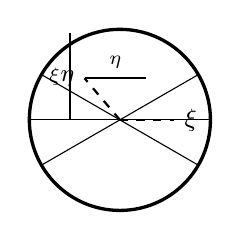
\begin{tikzpicture}[scale=1.15]
\draw[very thick] (0,0) circle (1);
\draw (-1,0) -- (1,0);
\draw (-0.866,-0.5) -- (0.866,0.5);
\draw (-0.866,0.5) -- (0.866,-0.5);
\draw[dashed,thick] (0,0) -- (0.6,0) node[right] {\small $\xi$};
\draw[dashed,thick] (0,0) -- (-0.39,0.459) node[left] {\small $\eta$};
\draw[thick] (-0.55,0) -- (-0.55,0.958);
\draw[thick] (-0.39,0.459) -- (0.29,0.459);
\draw[thick] (-0.39,0.459) -- (0.29,0.459) node[above,pos=0.5] {\scriptsize $\eta$};
\draw[thick] (-0.55,0) -- (-0.55,0.958) node[left,pos=0.5] {\scriptsize $\xi$};
\end{tikzpicture}
\caption{平面上的极坐标。沿 $\theta$ 方向走，$\hat r$ 与 $\hat\theta$ 的方向都在变；所以对矢量分量直接求偏导，会把「基矢量的变化」误算成「矢量本身的变化」。Christoffel 符号正是用来补偿这一项的。}
\end{figure}
